\documentclass{beamer}

\usepackage{ccf_beamer_macros}
\usepackage{tikz}
\usepackage{hyperref}


%%%%%%%%%%%%%%%%%%%%%%%%%%%%%%%%%%%%%%%%%%%%%%%%%%%%%%%%
%   begin document
%%%%%%%%%%%%%%%%%%%%%%%%%%%%%%%%%%%%%%%%%%%%%%%%%%%%%%%%

% You can fiddle with the vspace argument after the title, and then below in the first frame where the graphic is placed, to place the title and other titlepage information so that it doesn't overlap with the image in an awkward way
\title{Biostatistics: The New Frontier \vspace{1.9cm}} % this vspace controls the space between the title and the author
\author{Grade A. Author\\
Department of Quantitative Health Sciences}

\date[]{
January 1, 2021 \\
}


\titlegraphic

\begin{document}	


%%%%%%%%%%%%%%%%%%%%%%%%%%%%%%%%%%%%%%%%%%%%%%%%%%%%%%%%
%  create title slide with image background
%%%%%%%%%%%%%%%%%%%%%%%%%%%%%%%%%%%%%%%%%%%%%%%%%%%%%%%%

% This creates a custom footline argument for the first slide only, that doesn't include the page numbering, then we reset the frame counter to 0 after the first slide and the default footline argument from the macros will place page numbers in the form of x of xx on the remaining slides 
\bgroup
\makeatletter
\setbeamertemplate{footline}{
  \begin{beamercolorbox} {section in head/foot} 
\vskip1pt ~
  \hspace{2mm}
  
\includegraphics[width=.25\textwidth]{./figs/CC_c}
  ~\vskip5pt
  \end{beamercolorbox}
}
\makeatother
\begin{frame}
  \tikz [remember picture,overlay]
    \node at
        ([xshift=-4.8cm, yshift = 6cm]current page.south) 
        %or: (current page.center)
        {
\includegraphics[height=\textheight]{./figs/CC_Multiplicity_Blue_2tint}};
        \vspace{0.8cm} % this vspace argument controls the spacing of the title from the top of the slide
     \titlepage
\end{frame}
\egroup
\setcounter{framenumber}{0}


%%%%%%%%%%%%%%%%%%%%%%%%%%%%%%%%%%%%%%%%%%%%%%%%%%%%%%%%
% actual slides
%%%%%%%%%%%%%%%%%%%%%%%%%%%%%%%%%%%%%%%%%%%%%%%%%%%%%%%%

\begin{frame}{Just some text}

Lots of people have never heard of biostatistics. Time to spread the word.

\end{frame}


%%%%%%%%%%%%%%%%%%%%%%%%%%%%%%%%%%%%%%%%%%%%%%%%%%%%%%%%


\begin{frame}{Enumerated lists}

\begin{enumerate}
	\item First things first
	\begin{enumerate}
		\item I have a lot to say about biostatistics
		\item Just you wait!
	\end{enumerate}
	\item And then, a second thing
\end{enumerate}

\end{frame}


%%%%%%%%%%%%%%%%%%%%%%%%%%%%%%%%%%%%%%%%%%%%%%%%%%%%%%%%


\begin{frame}{Bulleted lists}

\begin{itemize}
	\item The goal is to learn about biostatistics
	\begin{itemize}
		\item Models
		\item Predictions
	\end{itemize}
	\item Then we'll move on to other topics
\end{itemize}

\end{frame}


%%%%%%%%%%%%%%%%%%%%%%%%%%%%%%%%%%%%%%%%%%%%%%%%%%%%%%%%


\begin{frame}{Inserting a figure}

Here's a picture of the Taussig Cancer Center

\begin{figure}[t]
    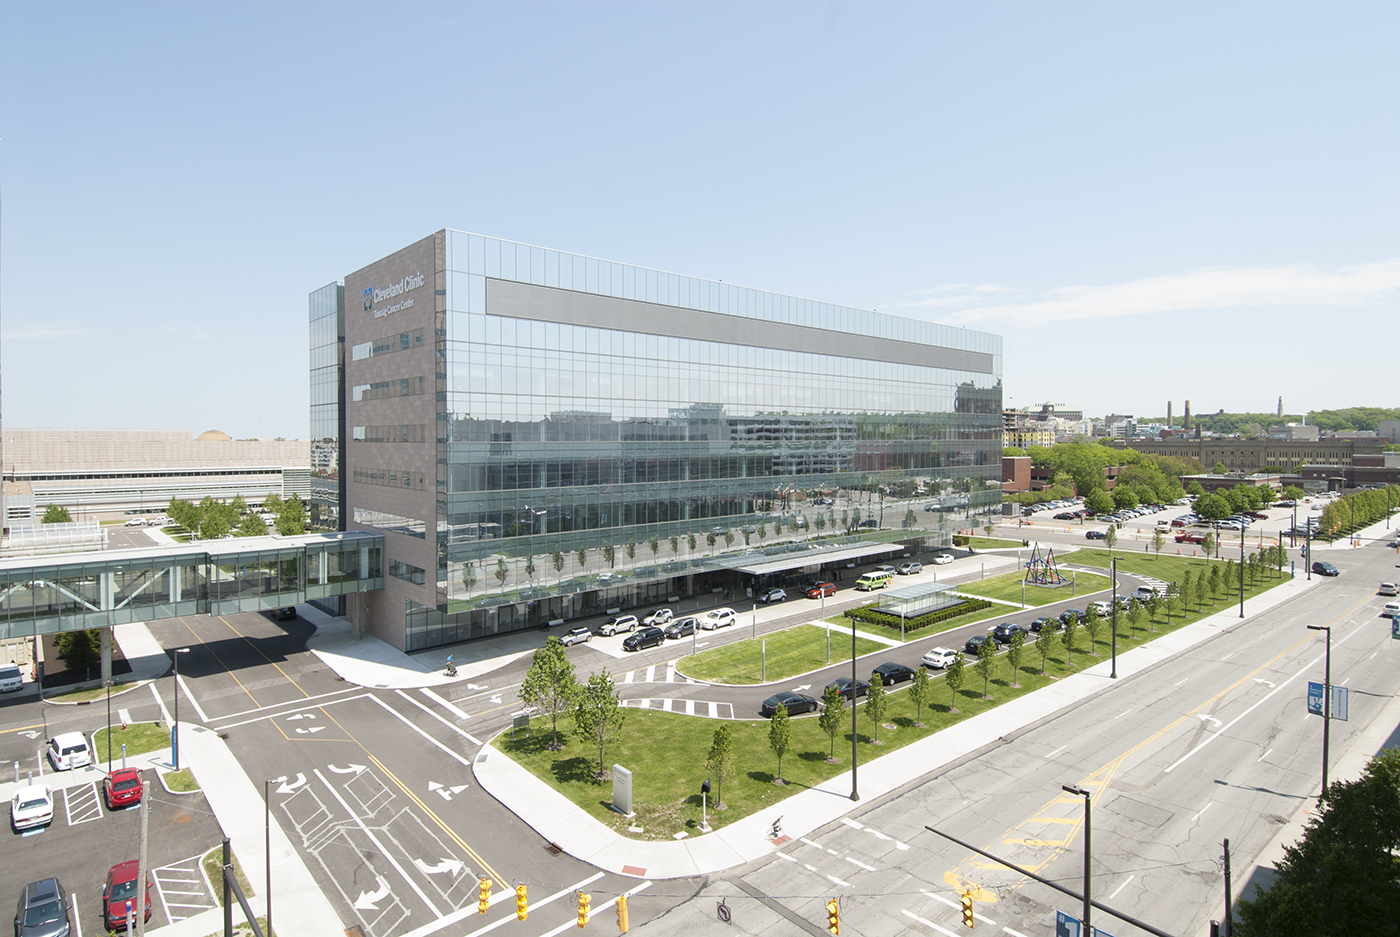
\includegraphics[width=.8\textwidth]{./figs/taussig-cancer-center_05-16-17}  
\end{figure}

\end{frame} 

\begin{frame}{Words, bullets, and equations}

Given some data $y, x_1, x_2, \ldots x_p$, we are interesting finding a likely value for $y$ given the value of predictors $x  \equiv x_1, x_2, \ldots x_p$.
\begin{itemize}
	\item Here, $y$ is continuous. (Called outcome, response, ``dependent variable").
	\item The $x$'s can be continuous, binary, categorical. (Called predictor, covariate, ``independent variable").
	\item We want $E(y | x) = f(x)$; we observe $y = f(x) + \epsilon$.
\end{itemize}

\end{frame}


%%%%%%%%%%%%%%%%%%%%%%%%%%%%%%%%%%%%%%%%%%%%%%%%%%%%%%%%


\begin{frame}[fragile]{Side by side figures}

On the left is incorrect mask use! Cover your nose, like on the right.

\begin{figure}[h]
  \centering
     \begin{tabular}{cc}
       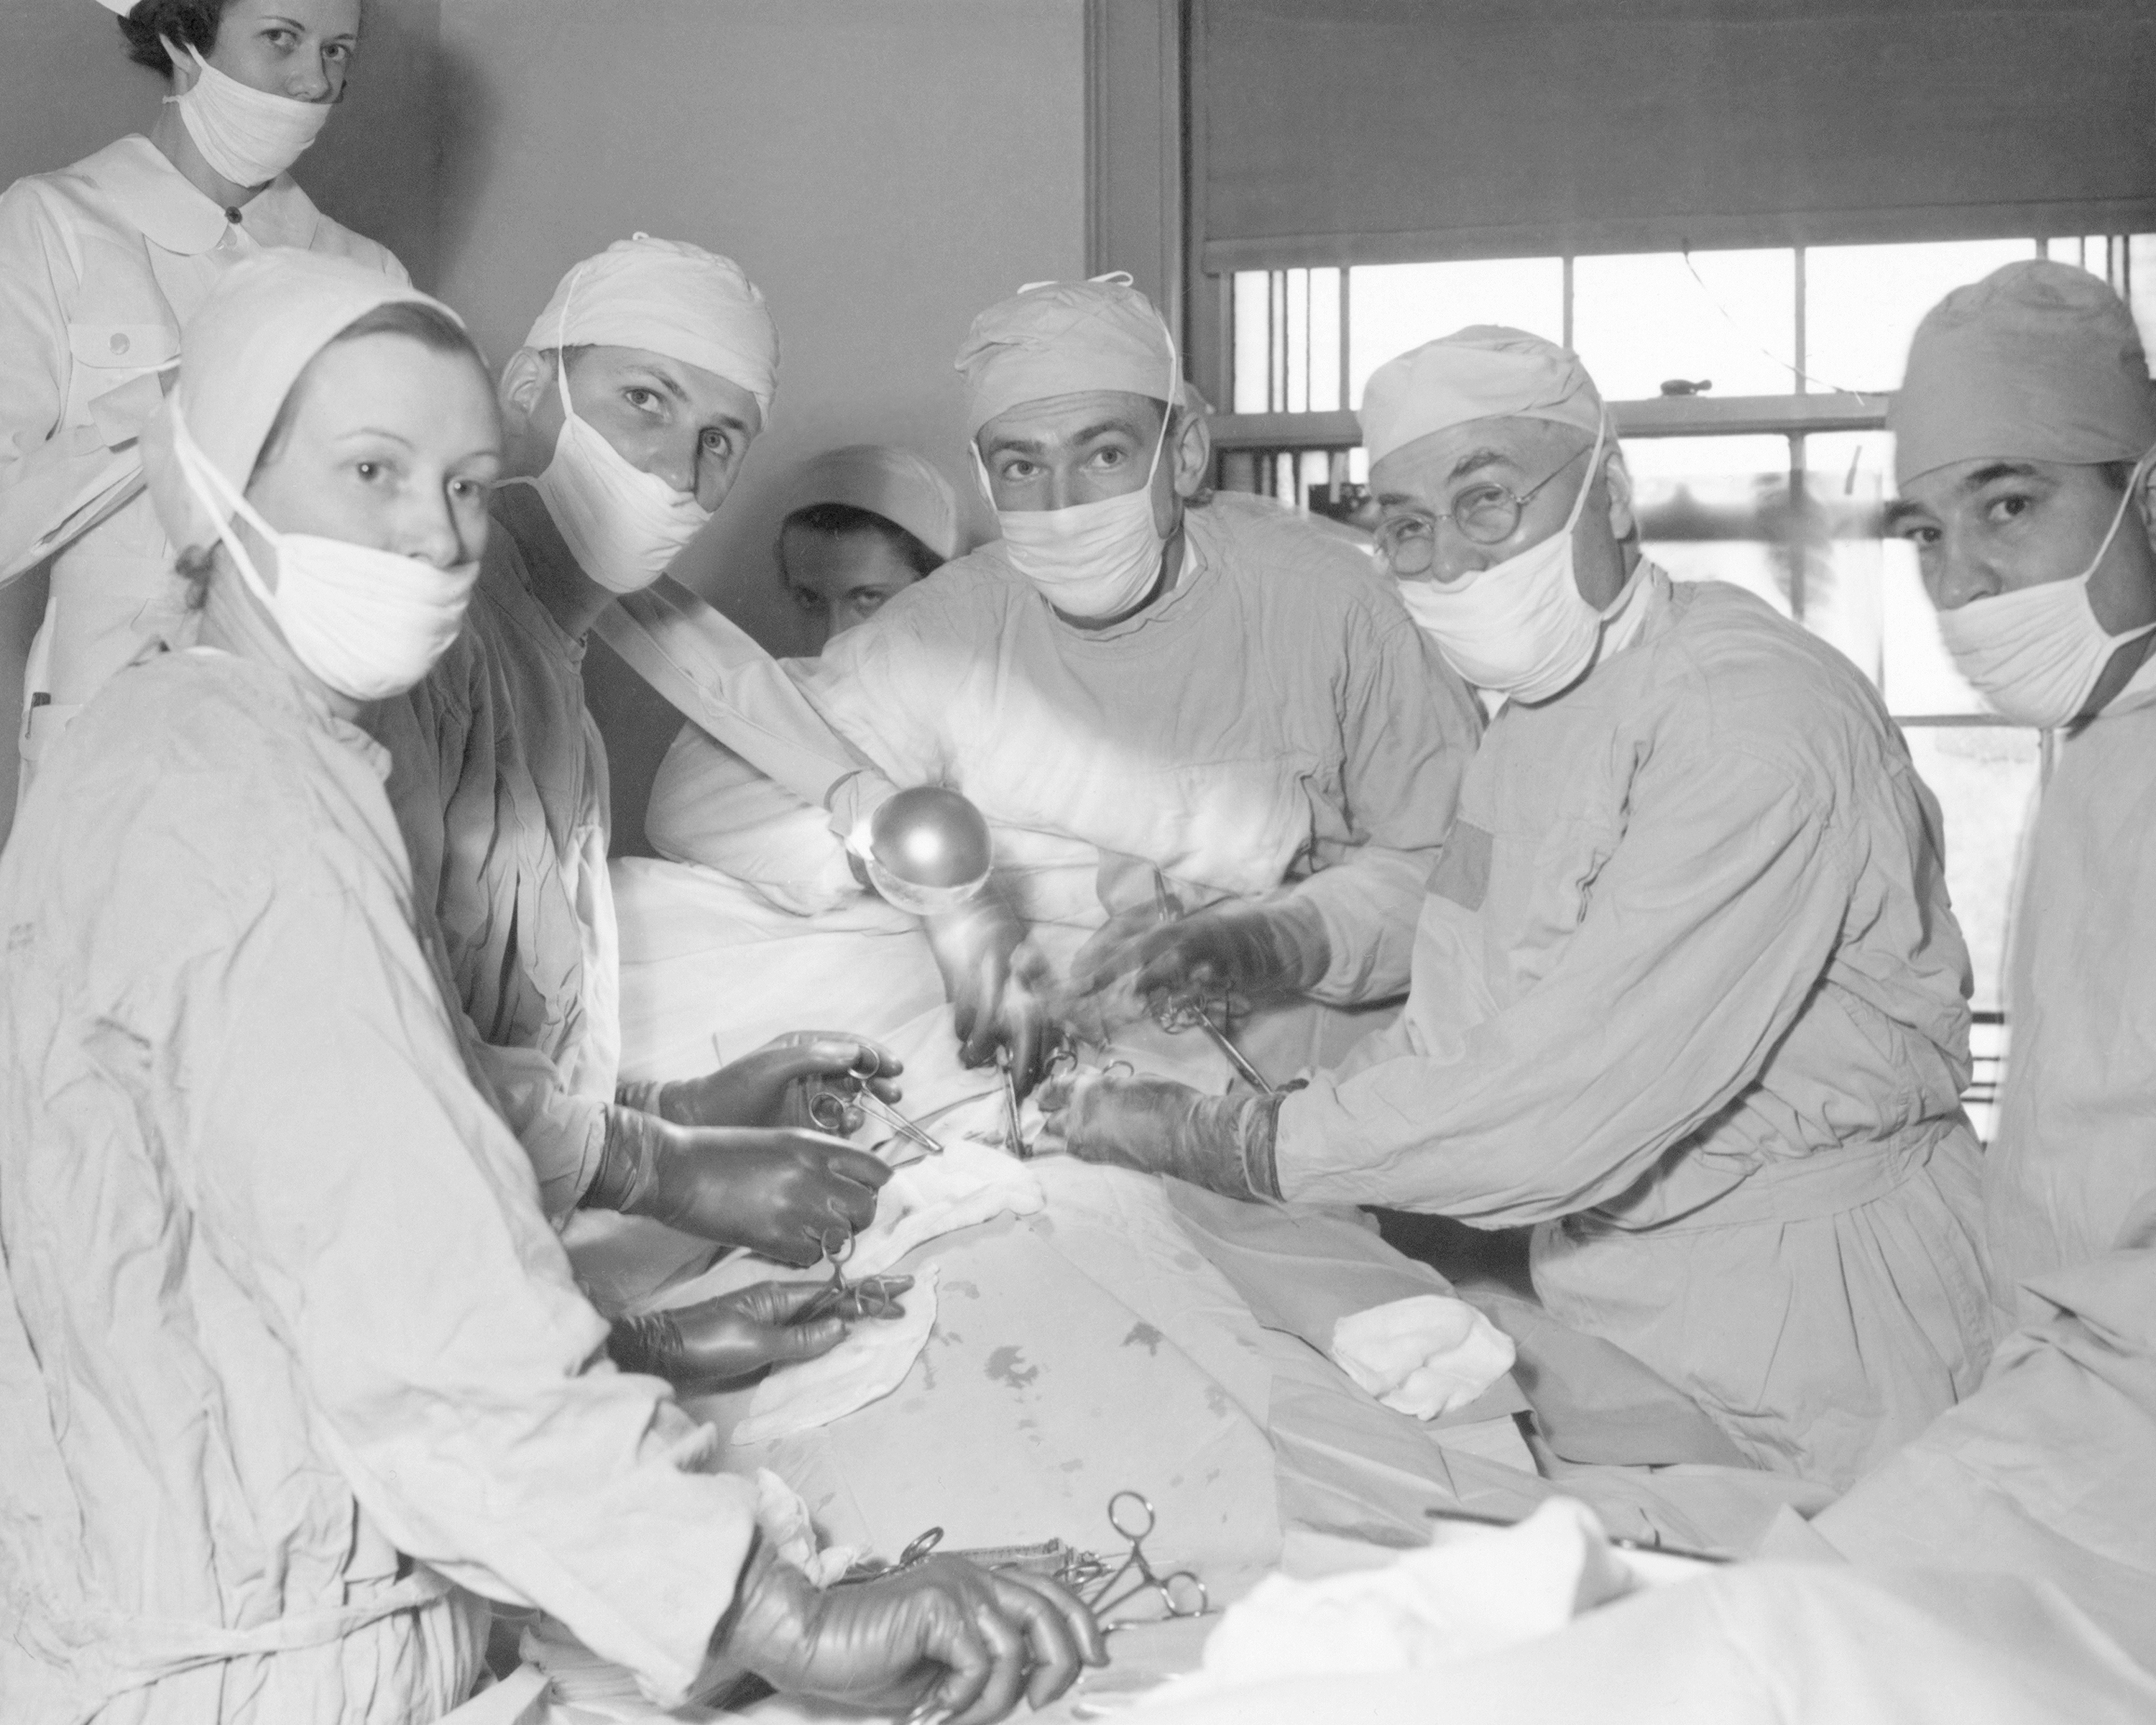
\includegraphics[width=.4\textwidth]{./figs/a0104} &
       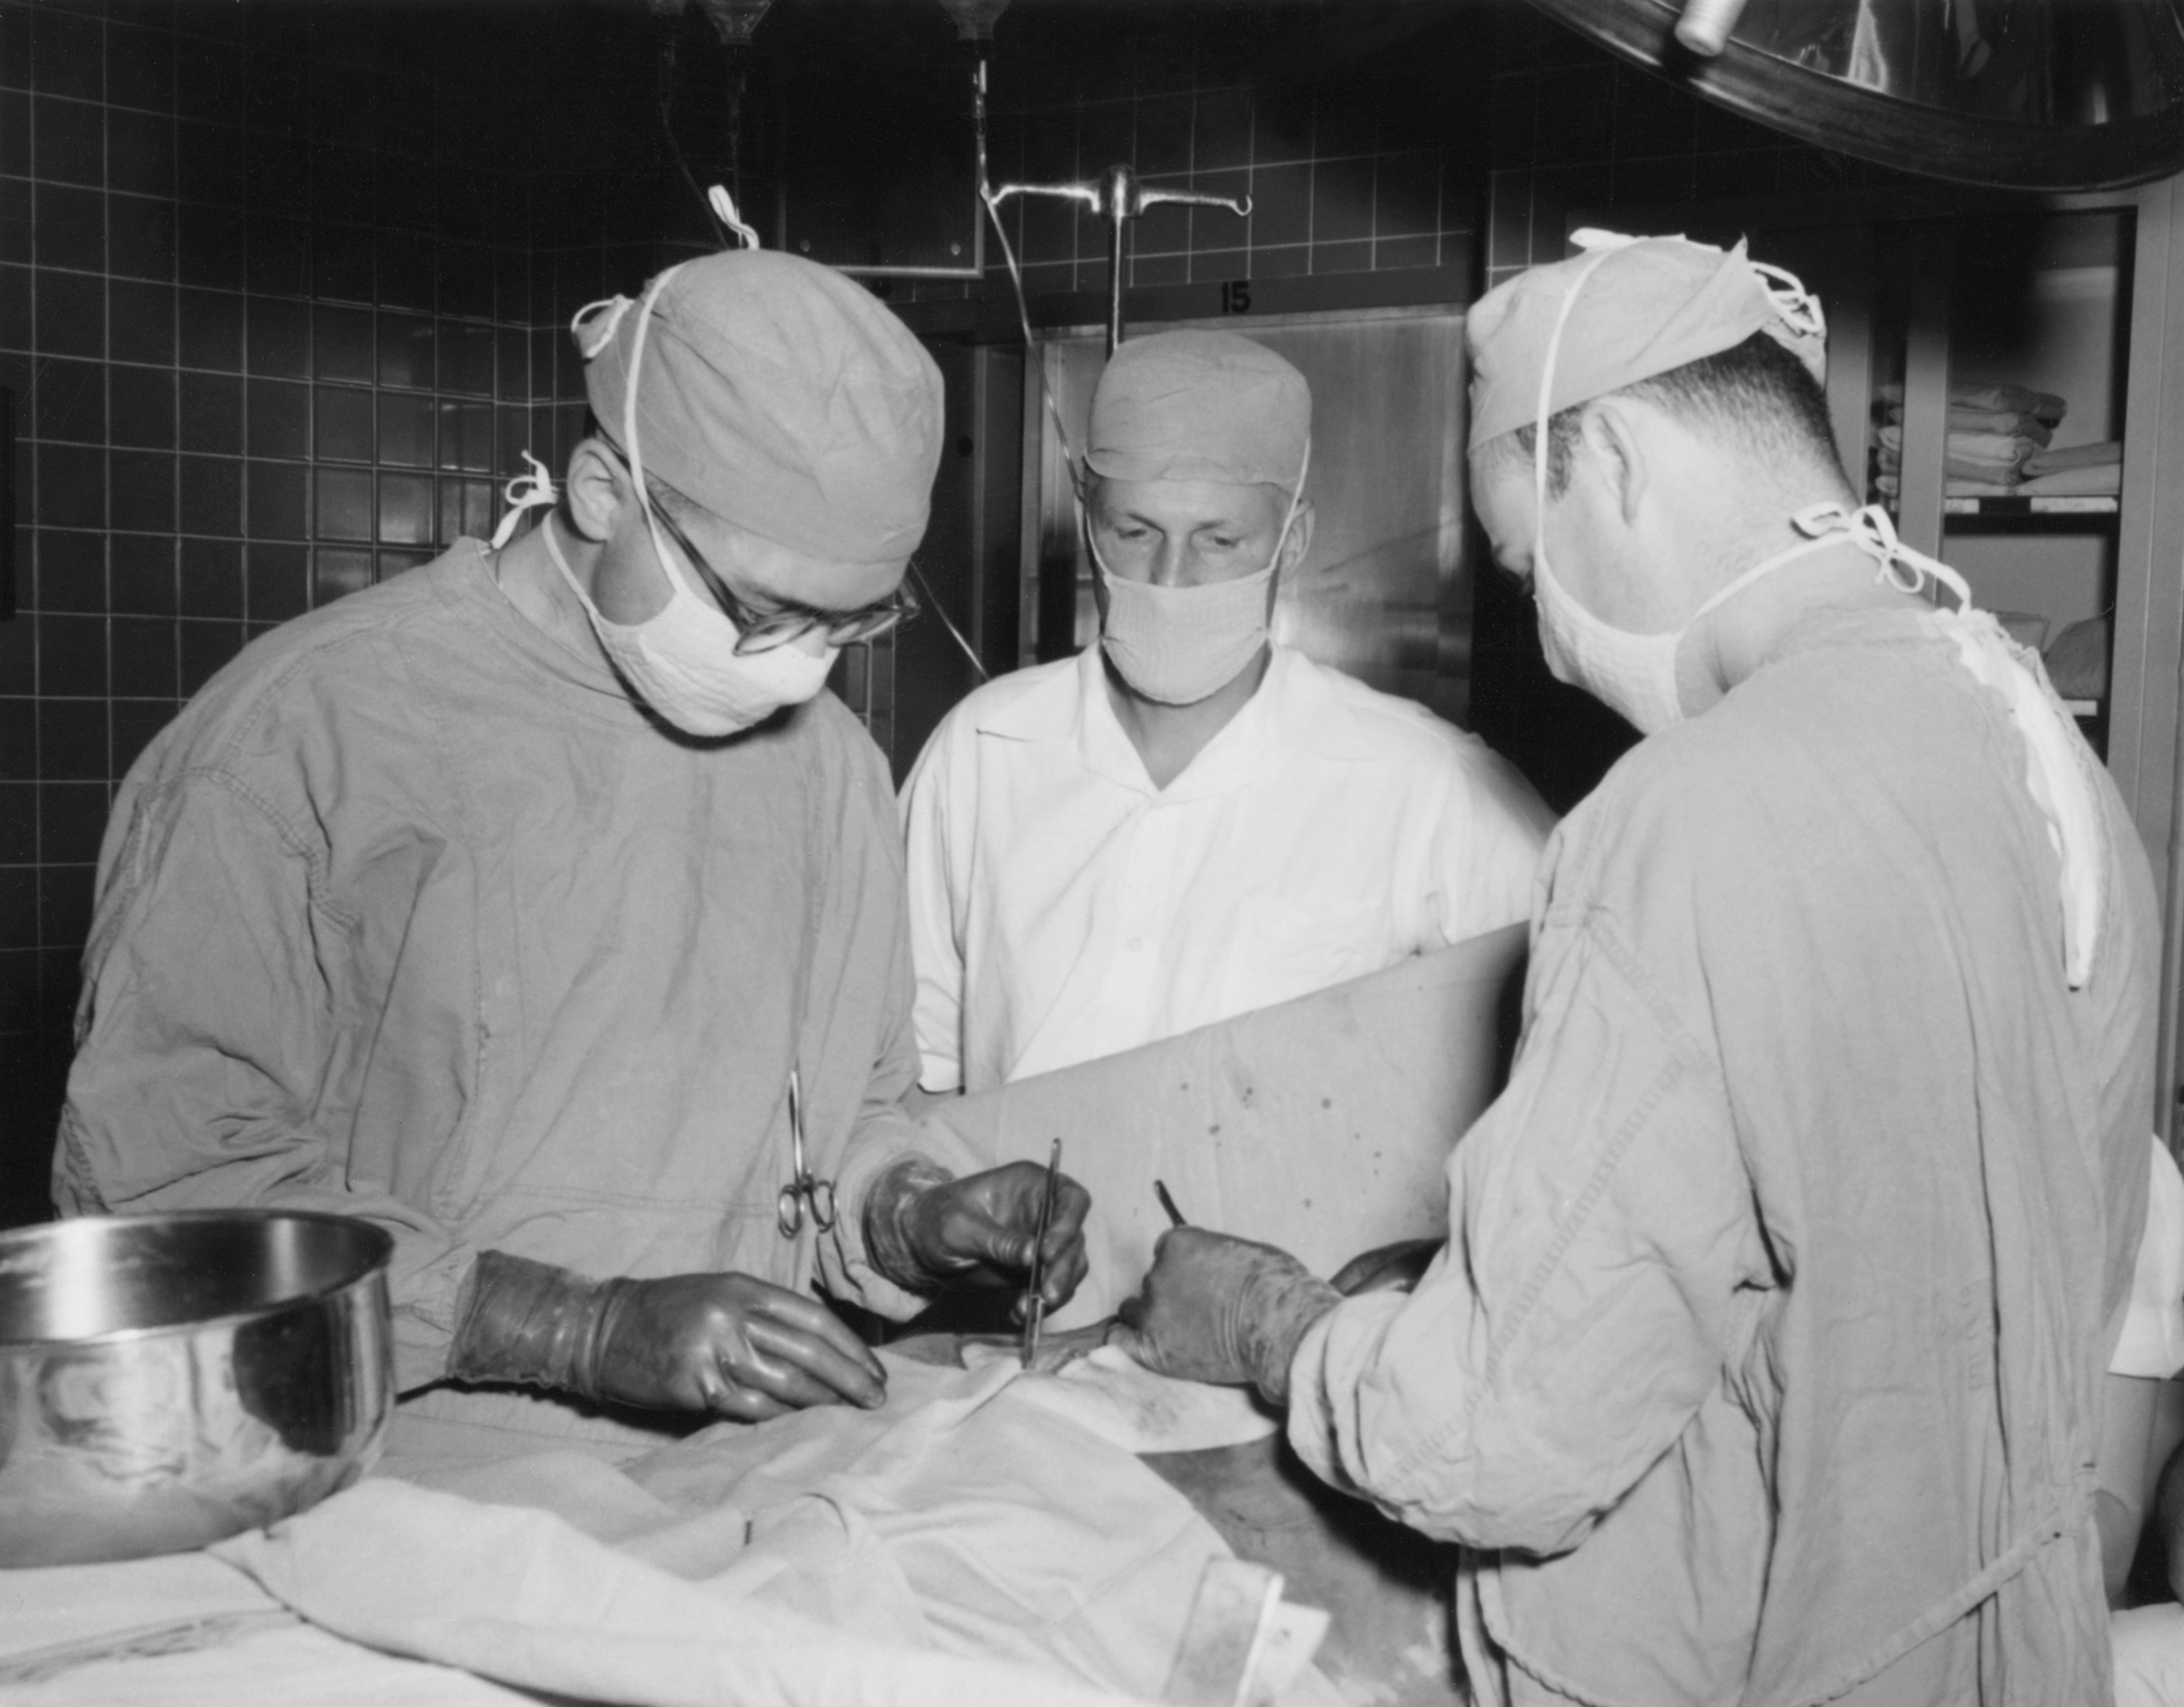
\includegraphics[width=.4\textwidth]{./figs/a0341}
     \end{tabular}
\end{figure}

\end{frame}


%%%%%%%%%%%%%%%%%%%%%%%%%%%%%%%%%%%%%%%%%%%%%%%%%%%%%%%%


\begin{frame}{Inline equations and nested lists}

A linear regression model is a particular type of parametric regression.

\begin{itemize}
	\item Assume $f(x; \beta) = \beta_0 + \beta_1 x_1 + \beta_2 x_2 + \ldots$
	\item Focus is on $\beta_0, \beta_1, \ldots$
	\item ``Linear" refers to the $\beta$'s, not the $x$'s: 
	\begin{itemize}
		\item $f(x) = \beta_0 + \beta_1 x + \beta_2 x^2$ is a linear model
		\item $f(x) = \beta_0 + x^{\beta_1}$ is not
		\item $f^{*}(x) = \beta_0^{*} + \beta_1 x^{*}$
	\end{itemize}
\end{itemize}

\end{frame}


%%%%%%%%%%%%%%%%%%%%%%%%%%%%%%%%%%%%%%%%%%%%%%%%%%%%%%%%


\begin{frame}[fragile]{Code blocks using verbatim}

\tiny
\begin{verbatim}
> lrmod <- lm(Sepal.Length ~ Species, data = iris)
> summary(lrmod)

Call:
lm(formula = Sepal.Length ~ Species, data = iris)

Residuals:
    Min      1Q  Median      3Q     Max 
-1.6880 -0.3285 -0.0060  0.3120  1.3120 

Coefficients:
                  Estimate Std. Error t value Pr(>|t|)    
(Intercept)         5.0060     0.0728  68.762  < 2e-16 ***
Speciesversicolor   0.9300     0.1030   9.033 8.77e-16 ***
Speciesvirginica    1.5820     0.1030  15.366  < 2e-16 ***
---
Signif. codes:  0 ‘***’ 0.001 ‘**’ 0.01 ‘*’ 0.05 ‘.’ 0.1 ‘ ’ 1

Residual standard error: 0.5148 on 147 degrees of freedom
Multiple R-squared:  0.6187,	Adjusted R-squared:  0.6135 
F-statistic: 119.3 on 2 and 147 DF,  p-value: < 2.2e-16
\end{verbatim}

\end{frame}


%%%%%%%%%%%%%%%%%%%%%%%%%%%%%%%%%%%%%%%%%%


\begin{frame}[fragile]{CCF plot colors}

\small
It's easy to make plots using the Cleveland Clinic brand colors in \verb!R!. 

Check out this website for details: 
\url{http://www.emilyzabor.com/ezfun/articles/ccf_color_palette.html}.

\begin{figure}
    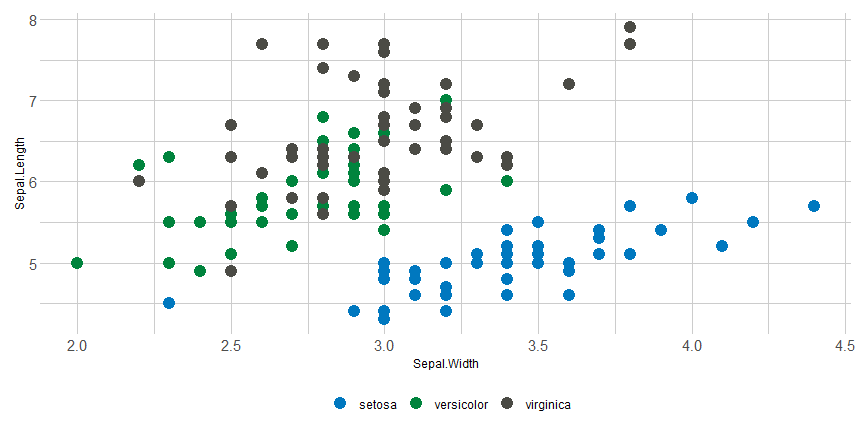
\includegraphics[scale=0.45]{./figs/example_ggplot}  
\end{figure}

\end{frame}


%%%%%%%%%%%%%%%%%%%%%%%%%%%%%%%%%%%%%%%%%%%%%%%%%%%%%%%%


\end{document}
